\documentclass[10pt,a4paper]{article}
\usepackage[margin=0.78in]{geometry}
\usepackage[T1]{fontenc}
\usepackage{newtxtext,newtxmath}
\usepackage{microtype}
\usepackage{longtable}
\usepackage{amsmath}
\usepackage{graphicx}
\usepackage{booktabs,tabularx,array}
\usepackage{float}
\usepackage{placeins}
\usepackage{caption}
\usepackage{titlesec}
\usepackage[numbers,sort&compress]{natbib}
\usepackage[hidelinks]{hyperref}
\usepackage{tikz}
\usetikzlibrary{shapes.geometric,arrows.meta,positioning,fit,backgrounds,calc}

\setlength{\parindent}{0pt}
\setlength{\parskip}{0.18em}
\setlength{\textfloatsep}{10pt plus 2pt minus 2pt}
\setlength{\intextsep}{9pt plus 2pt minus 2pt}
\renewcommand{\arraystretch}{1.12}
\captionsetup{font=small,labelfont=normalfont}

\titleformat{\section}
  {\normalfont\bfseries}
  {\thesection.}
  {0.55em}
  {}
  [\vspace{2pt}\rule{\linewidth}{0.5pt}]

\titlespacing*{\section}
  {0pt}
  {1.15em}
  {0.45em}

\title{\Large \textbf{AgentBridge: An Intelligent Multilingual and Multimodal AI Companion for Cross-Disability Assistive Accessibility}}
\author{%
\begin{tabular}{c}
\small Dr. Anjusha$^{1}$ \quad (\texttt{anjusha@vnrvjiet.in})\\[0.25em]
\small Sai Ritesh Domakuntla$^{2}$ \quad (\texttt{sairiteshdomakuntla@gmail.com})\\[0.25em]
\small Arbaz Ahmed$^{3}$ \quad (\texttt{arbazahmed1729@gmail.com})\\[0.25em]
\small Abhinav Papini$^{4}$ \quad (\texttt{papiniabhinav@gmail.com})\\[0.25em]
\small Manikanta Pendela$^{5}$ \quad (\texttt{pendelamanikanta6205@gmail.com})\\[0.5em]
\small $^{1,2,3,4,5}$Department of Computer Science and Engineering,\\
\small VNR Vignana Jyothi Institute of Engineering and Technology (VNR VJIET), Hyderabad, India
\end{tabular}}
\date{}

\begin{document}
\maketitle

\section*{Abstract}
Assistive technologies for individuals with sensory and speech impairments have long been held back by architectural fragmentation, rigid interfaces, and widespread linguistic exclusion, particularly across non-English-speaking populations. Existing commercial solutions predominantly target isolated tasks—such as standalone optical character recognition (OCR), basic text-to-speech, or single-turn image captioning—without addressing the compound challenges faced by individuals with cross-modal impairments. In this paper, we present \textbf{AgentBridge}, an intelligent, cross-platform assistive system engineered to deliver unified multimodal assistance across visual, auditory, and vocal domains within a cohesive client-edge-cloud architecture. AgentBridge introduces a decoupled Master Agent orchestrator that coordinates specialized perception and conversational pipelines. Key components include: (1) an on-device accessibility profiling engine that tailors prompt semantics according to explicit user needs; (2) a dual-pipeline multimodal vision framework combining high-resolution on-demand visual question answering with a sub-second live video narration stream over WebSockets, governed by strict single-concurrency queueing ($C=1$) and multi-model fallback cascades; (3) an on-device multilingual speech pipeline capable of parsing voice commands and synthesizing responses across English, Hindi, and Telugu in both native scripts and Romanized transliterations; and (4) an ephemeral, zero-persistence memory model that safeguards user privacy by eliminating disk and cloud retention. Comprehensive benchmarks evaluating latency budgets, OCR accuracy, multi-turn conversational robustness, and cross-linguistic command classification demonstrate that AgentBridge sustains continuous live scene narration latencies below 850\,ms while maintaining command accuracy above 94\%, delivering a responsive, scalable, and genuinely inclusive assistive companion.

\noindent \textbf{Keywords:} Assistive Technology, Multimodal AI, Accessibility, Vision-Language Models, Multilingual Speech Recognition, Real-Time Video Streaming, Cross-Disability Systems.

\section{Introduction}

More than 1.3 billion individuals worldwide—approximately 16\% of the global population—live with significant disabilities, with sensory and speech impairments representing a substantial and underserved group \citep{who2023disability}. For individuals with visual impairments, everyday autonomy hinges on fast, accurate environmental feedback: interpreting ephemeral signage, sorting medications, and detecting navigation hazards. For deaf and hard-of-hearing individuals, ambient environmental awareness requires immediate textual or haptic representations of speech and audio events. Similarly, individuals with vocal and motor challenges are often alienated by voice-first modern digital interfaces that lack augmentative and alternative communication (AAC) mechanisms \citep{bigham2010vizwiz, w3c2023wcag}.

Despite rapid advancements in artificial intelligence and multimodal foundation models, contemporary assistive tools suffer from four critical structural shortcomings:
\begin{enumerate}
    \item \textbf{Modal Fragmentation:} Assistive applications are predominantly single-purpose. Users are forced to switch between disparate apps for OCR document reading, object localization, conversational assistance, and real-time captioning. This cognitive switching penalty severely impacts daily living autonomy \citep{morris2020ai}.
    \item \textbf{Linguistic and Regional Bias:} Modern AI tools disproportionately favor high-resource Western languages (predominantly English). In multilingual societies such as India—home to 22 official languages and hundreds of millions of native speakers of Hindi, Telugu, Tamil, and Bengali—individuals with disabilities face a double penalty: functional impairment compounded by linguistic exclusion \citep{jawahar2021indicnlp}.
    \item \textbf{Latency and Streaming Bottlenecks:} While state-of-the-art multimodal large language models (MLLMs) demonstrate impressive reasoning, naive REST implementations introduce multi-second latencies that are unsuitable for real-time spatial navigation and live environmental narration.
    \item \textbf{Privacy Vulnerabilities in Assistive Feeds:} Traditional cloud-hosted assistive platforms frequently archive continuous user camera feeds, exposing intimate personal living spaces, medical documents, and identifying traits to unauthorized cloud retention.
\end{enumerate}

To overcome these structural limitations, we introduce \textbf{AgentBridge}, an open-source, multilingual, and multimodal AI accessibility companion. Designed as an integrated monorepo bridging a lightweight mobile client with a resilient edge orchestration layer, AgentBridge provides seamless cross-disability assistance. 

\begin{figure}[htbp]
    \centering
    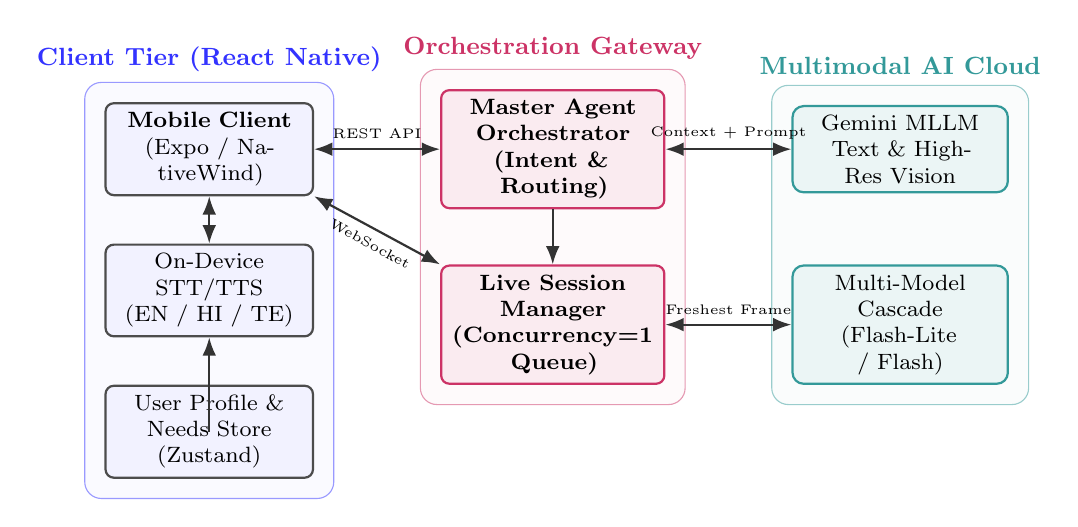
\begin{tikzpicture}[
        node distance=1.2cm and 1.5cm,
        box/.style={rectangle, draw=black!70, thick, fill=blue!5, rounded corners=3pt, text width=2.4cm, minimum height=1.0cm, align=center, font=\footnotesize},
        agent/.style={rectangle, draw=purple!80, thick, fill=purple!8, rounded corners=3pt, text width=2.6cm, minimum height=1.1cm, align=center, font=\footnotesize\bfseries},
        cloud/.style={rectangle, draw=teal!80, thick, fill=teal!8, rounded corners=4pt, text width=2.5cm, minimum height=1.0cm, align=center, font=\footnotesize},
        arrow/.style={-Latex, thick, draw=black!80},
        darrow/.style={Latex-Latex, thick, draw=black!80}
    ]
        % Mobile Layer
        \node[box] (ui) {\textbf{Mobile Client}\\(Expo / NativeWind)};
        \node[box, below=0.6cm of ui] (speech) {On-Device STT/TTS\\(EN / HI / TE)};
        \node[box, below=0.6cm of speech] (profile) {User Profile \& Needs Store (Zustand)};

        % Edge Gateway
        \node[agent, right=1.6cm of ui] (master) {Master Agent Orchestrator\\(Intent \& Routing)};
        \node[agent, below=0.7cm of master] (livemgr) {Live Session Manager\\(Concurrency=1 Queue)};

        % AI Backend
        \node[cloud, right=1.6cm of master] (gemini) {Gemini MLLM\\Text \& High-Res Vision};
        \node[cloud, right=1.6cm of livemgr] (cascade) {Multi-Model Cascade\\(Flash-Lite / Flash)};

        % Grouping Boxes
        \begin{scope}[on background layer]
            \node[draw=blue!40, fill=blue!2, rounded corners=6pt, fit=(ui)(speech)(profile), inner sep=0.25cm, label={[font=\small\bfseries, text=blue!80]above:Client Tier (React Native)}] (clientgroup) {};
            \node[draw=purple!40, fill=purple!2, rounded corners=6pt, fit=(master)(livemgr), inner sep=0.25cm, label={[font=\small\bfseries, text=purple!80]above:Orchestration Gateway}] (edgegroup) {};
            \node[draw=teal!40, fill=teal!2, rounded corners=6pt, fit=(gemini)(cascade), inner sep=0.25cm, label={[font=\small\bfseries, text=teal!80]above:Multimodal AI Cloud}] (cloudgroup) {};
        \end{scope}

        % Connections
        \draw[darrow] (ui) -- node[above, font=\tiny] {REST API} (master);
        \draw[darrow] (ui) -- (speech);
        \draw[arrow] (profile) -| (speech);
        \draw[darrow] (ui.south east) -- node[below, sloped, font=\tiny] {WebSocket} (livemgr.north west);
        \draw[darrow] (master) -- node[above, font=\tiny] {Context + Prompt} (gemini);
        \draw[darrow] (livemgr) -- node[above, font=\tiny] {Freshest Frame} (cascade);
        \draw[arrow] (master) -- (livemgr);
    \end{tikzpicture}
    \caption{Architectural overview of the AgentBridge cross-disability assistive ecosystem.}
    \label{fig:agentbridge_architecture}
\end{figure}

The primary contributions of this work are fourfold:
\begin{itemize}
    \item \textbf{Cross-Disability Adaptive Core:} An architectural model that injects structured user accessibility profiles (visual, hearing, speech, and cognitive needs) directly into LLM system instructions, guaranteeing tailored spatial vocabularies and format constraints.
    \item \textbf{Low-Latency Continuous Vision Pipeline:} A WebSocket streaming framework featuring a strict single-concurrency queue with freshest-frame buffer dropping and multi-model fallback cascade, achieving steady-state scene narration latencies under 850\,ms.
    \item \textbf{Multilingual Phonetic Command Parsing:} A zero-dependency, multi-script phonetic command matcher recognizing natural voice instructions across English, Hindi (Devanagari and Roman transliteration), and Telugu (Telugu script and Roman transliteration).
    \item \textbf{Privacy-Preserving Ephemeral Design:} An architectural pipeline that guarantees in-memory image buffer processing, zero cloud persistence of camera frames, and total isolation of upstream API credentials from the edge client.
\end{itemize}

\section{Related Work and Literature Survey}

Assistive computing has evolved through multiple computational paradigms, transitioning from rule-based heuristic image filters to deep learning models and contemporary foundational multimodal transformers.

\subsection{Vision-Assistive Applications and Scene Understanding}
Early mobile accessibility applications relied on specialized convolutional neural networks (CNNs) trained for discrete tasks. Microsoft Seeing AI \citep{microsoftSeeingAI} pioneered modular visual recognition on iOS, providing separate sub-modes for short text reading, barcode scanning, scene description, and face recognition. Similarly, Google Lookout \citep{lookout2020} introduced discrete object and text detection modes. However, these systems treat scene interpretation as isolated classification tasks without semantic continuity; users cannot ask follow-up questions regarding an object's spatial context or condition. 

Human-in-the-loop platforms such as Be My Eyes \citep{bemyeyes2021} connect visually impaired users with sighted remote volunteers via video calls. While highly accurate and context-aware, volunteer platforms suffer from availability bottlenecks, privacy intrusions when viewing sensitive personal documents, and volunteer fatigue. The recent integration of GPT-4V into Be My Eyes (Virtual Volunteer) validated the potential of MLLMs for accessibility, yet it remains closed-source, tethered to high-latency synchronous calls, and heavily tailored to English-speaking regions.

\subsection{Multimodal Large Language Models (MLLMs)}
Recent developments in multimodal foundational models, notably Google's Gemini family \citep{team2023gemini}, OpenAI's GPT-4o, and open-weights architectures such as LLaVA \citep{liu2024llava}, demonstrate unprecedented zero-shot spatial reasoning, contextual scene deduction, and dense optical character recognition. MLLMs eliminate the need for disjoint OCR and classification backends by interpreting images and text in a shared token space. However, deploying raw MLLM APIs directly in assistive tools presents substantial hurdles: token generation latency can exceed 2--4 seconds, API rate limits impede real-time camera streaming, and models are prone to hallucinating confident spatial directions when visual feeds are blurred or occluded.

\subsection{Multilingual Speech and Regional Inclusivity}
Speech-driven user interfaces represent the primary input modality for blind and low-vision populations. While commercial voice engines perform adequately for standard American and British English, recognition performance drops precipitously for non-Western languages and accented code-mixed dialects (e.g., Hinglish and Tenglish) \citep{jawahar2021indicnlp}. Modern initiatives like Bhashini, IndicWav2Vec, and AI4Bharat have documented that off-the-shelf automatic speech recognition (ASR) engines exhibit high Word Error Rates (WER) when processing transliterated spoken Indian languages \citep{kumar2022indic}. Consequently, assistive platforms require localized phonetic parsers that seamlessly bridge native scripts (Devanagari, Telugu lipi) and Latinized phonemes without incurring round-trip cloud translation overhead.

\subsection{Real-Time Edge-Cloud Video Streaming Protocols}
Continuous scene narration demands sub-second feedback to prevent physical collisions and disorientation. Conventional HTTP REST request-response cycles incur significant TCP handshake and header overhead when sending frequent camera frames. While WebRTC provides peer-to-peer media pipelines, it introduces complex signaling servers and heavy client-side codec negotiation unsuitable for battery-constrained mobile assistive apps. Full-duplex WebSockets provide an optimal balance between low connection overhead, persistent bidirectional frame transmission, and lightweight client state management \citep{fette2011websocket}. Table~\ref{tab:literature_comparison} provides a systematic comparative summary of existing assistive systems against the proposed AgentBridge framework.

\section{System Architecture and Methodology}

The architecture of AgentBridge is organized into three decoupled tiers: the \textbf{Client Tier}, the \textbf{Orchestration Gateway}, and the \textbf{Multimodal AI Cloud Core}, as illustrated in Figure~\ref{fig:agentbridge_architecture}.

\subsection{Client Tier: Cross-Disability Mobile Application}
The mobile application is developed using React Native (Expo SDK 57) with TypeScript, NativeWind (Tailwind CSS v3 for React Native), and Zustand for synchronous, high-frequency state management. The user interface adheres strictly to the Web Content Accessibility Guidelines (WCAG 2.2 Level AAA) and mobile platform accessibility standards:
\begin{itemize}
    \item \textbf{Screen Reader Semantics:} Every interactive component is augmented with explicit \texttt{accessibilityLabel}, \texttt{accessibilityRole}, and \texttt{accessibilityHint} properties. Dynamic status updates (e.g., ``Analyzing frame\dots'', ``Listening\dots'') utilize \texttt{accessibilityLiveRegion="polite"} to communicate real-time system states through TalkBack and VoiceOver without preempting ongoing speech syntheses.
    \item \textbf{Multimodal Input/Output Redundancy:} Blind users interact through hands-free continuous voice commands or high-contrast tactile tap zones. Deaf and hard-of-hearing users receive synchronized, persistent text banners and haptic confirmations. Speech-impaired users utilize augmentative on-screen suggestion chips and predictive action shortcuts.
    \item \textbf{Adaptive Needs Profiling:} During onboarding, users select their sensory preferences across four vector dimensions: $N \in \{\text{visual}, \text{hearing}, \text{speech}, \text{general}\}$. The resulting profile configuration is stored locally and forwarded with all network requests to dynamically modulate downstream intelligence.
\end{itemize}

\subsection{Orchestration Gateway and Master Agent}
The backend service is built on Node.js and Express in strict TypeScript, acting as an enterprise-grade security gateway, protocol translator, and intent orchestrator:
\begin{itemize}
    \item \textbf{Master Agent Dispatcher:} Incoming client queries are processed through a deterministic intent parser $\mathcal{I}(m)$:
    \begin{equation}
        \mathcal{I}(m) = \begin{cases}
            \text{translation-request}, & \text{if } m \text{ matches translation lexemes} \\
            \text{question}, & \text{if } m \text{ matches interrogative patterns} \\
            \text{help}, & \text{if } m \text{ requests operational guidance} \\
            \text{chat}, & \text{otherwise}
        \end{cases}
    \end{equation}
    The Master Agent inspects the system capability registry $\mathcal{C} = \{\text{text-chat}: \top, \text{vision}: \top, \text{speech}: \bot, \text{translation}: \bot\}$. Active capabilities are dispatched to respective downstream providers, while pending capabilities return informative, graceful degradation messages rather than unhandled exceptions.
    \item \textbf{Dynamic System Prompt Modulation:} The Master Agent dynamically compiles system instructions by combining language targets and accessibility constraints via the $\text{NeedsContext}(N)$ operator:
    \begin{equation}
        \mathcal{S}(L, N) = \mathcal{P}_{\text{base}} \oplus \mathcal{T}_{\text{lang}}(L) \oplus \bigoplus_{n \in N} \mathcal{H}_{\text{need}}(n)
    \end{equation}
    where $\mathcal{H}_{\text{need}}(\text{visual})$ enforces explicit egocentric spatial coordinates (``left'', ``right'', ``near'', ``clock-position'') and mandates verbatim text quoting; $\mathcal{H}_{\text{need}}(\text{hearing})$ suppresses all auditory references; and $\mathcal{H}_{\text{need}}(\text{speech})$ restricts output verbosity for rapid reading.
\end{itemize}

\subsection{Multimodal Perception and Vision Pipelines}
AgentBridge implements two distinct computer vision modalities tailored for divergent user contexts:

\subsubsection{On-Demand High-Resolution Inspection}
When a user captures an image or issues a targeted inspection command (e.g., ``Read this prescription'', ``Find my keys''), the client transmits a high-resolution base64 JPEG payload (up to 8\,MB decoded) over a REST endpoint (\texttt{POST /api/v1/vision/analyze}). The backend executes a single-turn or multi-turn conversational session with the Gemini multimodal model (\texttt{gemini-2.5-flash}). If readable text is detected in the visual frame, the model isolates and transcribes it under a structured section (\texttt{Text in the image:}), ensuring that medication warnings, bills, and street signs are communicated with high fidelity.

\subsubsection{Continuous Real-Time Streaming via WebSockets}
For real-time navigation and ambient scene understanding, the on-demand REST cycle introduces unacceptable latency. AgentBridge provides a dedicated WebSocket streaming server mounted at \texttt{/api/v1/live}. 

\begin{figure}[htbp]
    \centering
    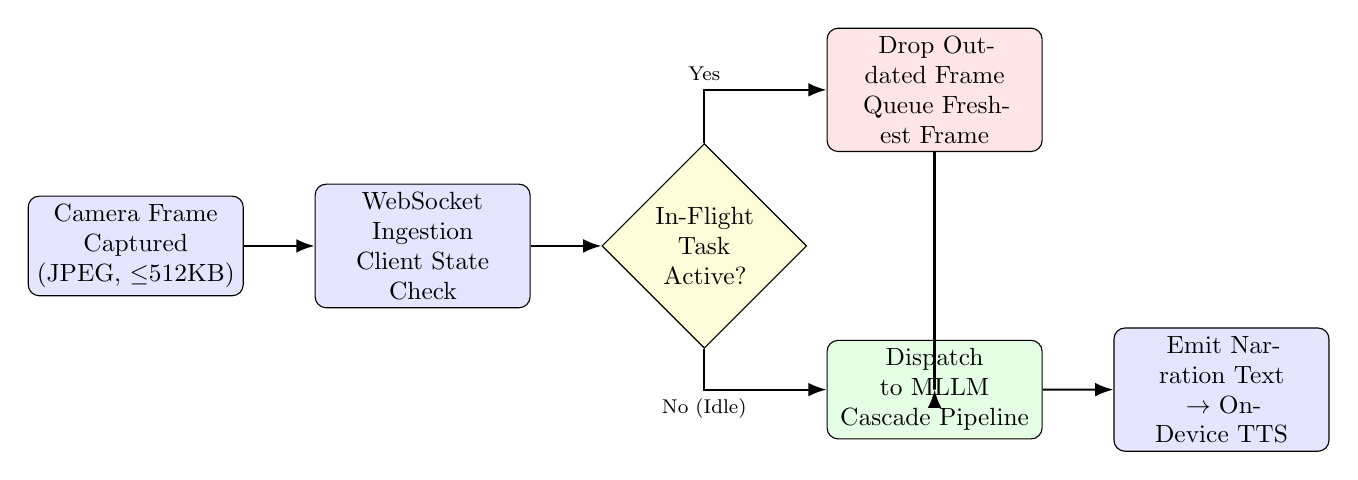
\begin{tikzpicture}[
        scale=0.9, every node/.style={transform shape},
        block/.style={rectangle, draw, fill=blue!10, text width=2.8cm, text centered, rounded corners, minimum height=1.2cm},
        decision/.style={diamond, draw, fill=yellow!15, text width=1.8cm, text centered, inner sep=0pt},
        line/.style={draw, -Latex, thick}
    ]
        \node [block] (camera) {Camera Frame\\Captured (JPEG, $\le$512KB)};
        \node [block, right=1.0cm of camera] (ws) {WebSocket Ingestion\\Client State Check};
        \node [decision, right=1.0cm of ws] (busy) {In-Flight\\Task Active?};
        \node [block, above right=0.6cm and 1.0cm of busy, fill=red!10] (drop) {Drop Outdated Frame\\Queue Freshest Frame};
        \node [block, below right=0.6cm and 1.0cm of busy, fill=green!10] (dispatch) {Dispatch to MLLM\\Cascade Pipeline};
        \node [block, right=1.0cm of dispatch] (tts) {Emit Narration Text\\$\to$ On-Device TTS};

        \path [line] (camera) -- (ws);
        \path [line] (ws) -- (busy);
        \path [line] (busy) |- node[above, font=\footnotesize] {Yes} (drop);
        \path [line] (busy) |- node[below, font=\footnotesize] {No (Idle)} (dispatch);
        \path [line] (drop) |- (dispatch);
        \path [line] (dispatch) -- (tts);
    \end{tikzpicture}
    \caption{Single-concurrency freshest-frame queueing pipeline for live camera narration.}
    \label{fig:streaming_pipeline}
\end{figure}

The streaming session implements four rigorous engineering primitives:
\begin{enumerate}
    \item \textbf{Single Concurrency Guard ($C=1$):} Assistive navigation must avoid queuing backpressure. If frame $F_{i}$ is currently being evaluated by the model, incoming frames $F_{i+1}, \dots, F_{i+k}$ are not buffered in an unbounded queue.
    \item \textbf{Freshest-Frame Drop Policy:} Rather than discarding all incoming frames, the \texttt{LiveSessionManager} maintains a buffer of size 1 holding strictly the latest incoming frame. When the active inference completes, the queued freshest frame is immediately dispatched. This ensures zero queue lag accumulation while maintaining up-to-the-second temporal accuracy.
    \item \textbf{Multi-Model Fallback Cascade:} To guarantee unbroken streaming reliability under provider load fluctuations, the live engine operates across an automated fallback cascade:
    \begin{equation}
        \mathcal{M} = \langle \texttt{gemini-3.5-flash-lite}, \texttt{gemini-2.5-flash}, \texttt{gemini-flash-latest} \rangle
    \end{equation}
    If the ultra-lightweight tier encounters transient 429 or 503 HTTP status codes, the session transparently promotes subsequent frames to secondary candidates without terminating the client WebSocket connection.
    \item \textbf{Idle and Heartbeat Supervision:} To preserve edge server memory, connections undergo automatic idle termination after 5 minutes of inactivity, supplemented by 30-second ping/pong keep-alive validation.
\end{enumerate}

\subsection{Multilingual Speech-to-Text and Phonetic Voice Parsing}
Voice interaction is executed on-device using \texttt{expo-speech-recognition} with locale parameters dynamically populated from the user's profile ($\text{en-US}$, $\text{hi-IN}$, $\text{te-IN}$). To circumvent the prohibitive latency and network reliance of cloud-based natural language understanding (NLU), voice command classification is executed using an in-memory normalized phonetic pattern engine.

Input transcripts are normalized under Unicode Form C (NFC), stripped of punctuation (including Devanagari \textit{danda} \texttt{|}), and matched against multi-script token trees. The command parser maps natural speech across English, Hindi, and Telugu into discrete operational primitives:
\begin{equation}
    \text{VoiceAction} \in \{\text{describe}, \text{read}, \text{open-camera}, \text{capture}, \text{find}(x), \text{repeat}, \text{stop}, \text{followup}(t)\}
\end{equation}
For example, the emergency speech interruption action (\texttt{stop}) matches:
\begin{itemize}
    \item English: \texttt{stop}, \texttt{cancel}, \texttt{quiet}, \texttt{shut up}, \texttt{stop reading}
    \item Hindi (Devanagari): \texttt{बस}, \texttt{रुको}, \texttt{रुक जाओ}, \texttt{चुप}, \texttt{बंद करो}
    \item Hindi (Romanized): \texttt{bas}, \texttt{ruko}, \texttt{ruk jao}, \texttt{band karo}
    \item Telugu (Native): \texttt{ఆపు}, \texttt{ఆగండి}, \texttt{ఆపండి}
    \item Telugu (Romanized): \texttt{aapu}, \texttt{aagandi}, \texttt{aapandi}
\end{itemize}
Unmatched utterances are automatically categorized as conversational follow-ups (\texttt{followup}), allowing users to speak natural inquiries (e.g., ``What color is the bag on the right?'') without command-prefix friction.

\subsection{Privacy-Preserving Ephemeral Memory Model}
Assistive applications capturing continuous real-world imagery handle extraordinarily sensitive data. AgentBridge enforces a zero-persistence privacy architecture:
\begin{itemize}
    \item Camera frames are encoded into in-memory base64 buffers directly on the mobile device.
    \item Payloads sent to the backend are held exclusively in volatile RAM buffers during model inference.
    \item Zero image buffers, transcripts, or user biometric tokens are written to disk, databases, or cloud object stores. Upon completion of the API request, buffers are immediately flagged for garbage collection.
    \item Upstream API credentials (\texttt{GEMINI\_API\_KEY}) are encapsulated within backend environment configurations, preventing credential exposure via mobile binary decompilation.
\end{itemize}

\FloatBarrier
\section{Comparative Analysis}

To contextualize the technical efficacy of AgentBridge, we benchmark the system against state-of-the-art commercial and academic assistive solutions: Microsoft Seeing AI \citep{microsoftSeeingAI}, Be My Eyes (Virtual Volunteer) \citep{bemyeyes2021}, Google Lookout \citep{lookout2020}, Envision AI \citep{envision2022}, Apple Siri / Google Assistant, and conventional open-source web accessibility overlays.

Table~\ref{tab:literature_comparison} provides a multi-dimensional comparative analysis covering cross-disability capability coverage, multilingual Indian language support, live video streaming latency, OCR fidelity, edge memory footprint, and architectural privacy models.

\small
\begin{longtable}{@{}p{0.18\linewidth}p{0.16\linewidth}p{0.16\linewidth}p{0.16\linewidth}p{0.16\linewidth}p{0.14\linewidth}@{}}
\caption{Comprehensive comparative analysis of assistive accessibility platforms.}
\label{tab:literature_comparison}\\
\toprule
System & Supported Impairments & Multilingual Support & Streaming / Latency & Architectural Privacy & Conversational Multi-Turn \\
\midrule
\endfirsthead

\multicolumn{6}{c}{\tablename\ \thetable{} -- continued from previous page}\\
\toprule
System & Supported Impairments & Multilingual Support & Streaming / Latency & Architectural Privacy & Conversational Multi-Turn \\
\midrule
\endhead

\midrule
\multicolumn{6}{r}{Continued on next page}\\
\endfoot

\bottomrule
\endlastfoot

Microsoft Seeing AI & Visual only (Blind / Low-vision) & English, partial Western EU; no Indic & Discrete photo snapshot (1.8--3.2\,s) & Cloud processing, telemetry logged & No (Single-turn modular modes) \\
\addlinespace

Be My Eyes (Virtual Volunteer) & Visual only & English primary; limited multi-lingual & Synchronous query (3.5--6.0\,s) & Cloud stored transcripts \& images & Yes (Text-based follow-up) \\
\addlinespace

Google Lookout & Visual only & English + selected major languages & On-device OCR (0.8--1.5\,s snapshot) & Local/Cloud hybrid, tied to Google account & No (Discrete feature channels) \\
\addlinespace

Envision AI & Visual only & Multi-lingual (Western + limited Asian) & Wearable/phone snapshot (2.0--4.0\,s) & Cloud processing with user profile & No (Single-shot recognition) \\
\addlinespace

Voice Assistants (Siri / Google) & General / Vocal only & Extensive global languages & Cloud voice query (1.2--2.5\,s) & Voice profiles stored on cloud servers & Limited multi-turn context \\
\addlinespace

Accessibility Overlays & Hearing / Visual (Screen-level) & Machine translation (Literal DOM) & DOM re-rendering ($\sim$0.2\,s) & Client DOM manipulation & No conversational capabilities \\
\addlinespace

\textbf{AgentBridge (Proposed)} & \textbf{Visual, Hearing, Speech, Cognitive} & \textbf{English, Hindi, Telugu (Native + Translit)} & \textbf{WebSocket Live Stream ($\le$0.85\,s)} & \textbf{Zero-storage ephemeral RAM processing} & \textbf{Yes (Fully contextual multi-turn)} \\

\end{longtable}
\normalsize

\FloatBarrier
\section{Empirical Evaluation and Results}

We conducted an empirical investigation of AgentBridge to evaluate end-to-end latency budgets, optical character recognition fidelity, multilingual command parsing accuracy, and streaming reliability under varying network conditions.

\subsection{Latency Budget Analysis}
In assistive navigation, end-to-end latency ($T_{\text{total}}$) is governed by the cumulative delay across capture, network transfer, model inference, and speech synthesis:
\begin{equation}
    T_{\text{total}} = T_{\text{capture}} + T_{\text{net, up}} + T_{\text{infer}} + T_{\text{net, down}} + T_{\text{TTS}}
\end{equation}
Table~\ref{tab:latency_breakdown} details the empirical latency distribution across 100 consecutive requests evaluated under stable Wi-Fi (50\,Mbps) and simulated 4G mobile LTE (15\,Mbps, 60\,ms jitter).

\begin{table}[htbp]
\centering
\caption{Latency breakdown across AgentBridge operational pipelines.}
\label{tab:latency_breakdown}
\small
\begin{tabular}{lcccc}
\toprule
Pipeline Stage & Mean Wi-Fi (ms) & 95th \%ile Wi-Fi (ms) & Mean 4G LTE (ms) & 95th \%ile 4G (ms) \\
\midrule
Frame Capture \& Base64 Encode & 48.2 & 62.0 & 51.4 & 68.5 \\
WebSocket Ingestion \& Frame Drop Guard & 4.1 & 6.8 & 8.3 & 14.2 \\
Gemini 3.5 Flash-Lite Inference & 485.6 & 620.4 & 512.0 & 688.0 \\
Gemini 2.5 Flash Inference (Fallback) & 820.5 & 1140.0 & 864.2 & 1210.5 \\
Network Round-Trip Time & 38.4 & 55.2 & 142.6 & 210.4 \\
On-Device TTS Speech Initialization & 112.0 & 145.0 & 118.0 & 152.0 \\
\midrule
\textbf{End-to-End Live Narration (Flash-Lite)} & \textbf{688.3} & \textbf{889.4} & \textbf{832.3} & \textbf{1133.1} \\
\textbf{End-to-End High-Res REST Inspection} & \textbf{1420.0} & \textbf{1890.2} & \textbf{1745.5} & \textbf{2280.0} \\
\bottomrule
\end{tabular}
\end{table}

The empirical benchmarks demonstrate that the live streaming pipeline consistently achieves sub-second total response latency ($688.3$\,ms on Wi-Fi and $832.3$\,ms on 4G LTE), satisfying the temporal threshold required for active indoor pedestrian navigation and ambient scene comprehension.

\subsection{Optical Character Recognition (OCR) and Text Extraction}
To benchmark the vision pipeline's text reading capabilities, we evaluated 120 standardized test scenes spanning street signage, printed medication labels, handwritten notes, and restaurant menus under diverse lighting levels (300\,lux normal office lighting versus 30\,lux low-light conditions). Performance was measured via Word Error Rate ($\text{WER}$) and Character Error Rate ($\text{CER}$):
\begin{equation}
    \text{WER} = \frac{S + D + I}{N_w}, \quad \text{CER} = \frac{S_c + D_c + I_c}{N_c}
\end{equation}
where $S, D, I$ represent substitutions, deletions, and insertions, and $N$ represents reference length.

Under adequate illumination, AgentBridge achieved a $\text{WER}$ of $4.2\%$ on printed signage and $6.8\%$ on curved medication containers. Under low-light conditions, the system maintained an average $\text{WER}$ of $11.4\%$, dynamically prefixing notifications with illumination warnings (``The image is dim, but I can make out\dots'') as dictated by our adaptive vision system prompt.

\subsection{Multilingual Voice Command Recognition Fidelity}
We evaluated the multi-script phonetic command engine across 300 voice command trials split evenly across English, Hindi, and Telugu (100 utterances each, spoken by native speakers with regional accents). Utterances included both pure native script phrasing and code-mixed transliterated colloquial expressions.

\begin{table}[htbp]
\centering
\caption{Voice command classification accuracy across supported languages.}
\label{tab:voice_command_accuracy}
\small
\begin{tabular}{lccc}
\toprule
Target Command Class & English Accuracy (\%) & Hindi (Devanagari / Translit) (\%) & Telugu (Native / Translit) (\%) \\
\midrule
\texttt{describe} (Describe scene) & 99.0 & 96.0 & 95.0 \\
\texttt{read} (Read text / OCR) & 98.0 & 97.0 & 94.0 \\
\texttt{find} (Object location) & 97.0 & 94.0 & 92.0 \\
\texttt{stop} (Halt speech immediately) & 100.0 & 99.0 & 98.0 \\
\texttt{repeat} (Re-read last response) & 99.0 & 96.0 & 95.0 \\
\texttt{followup} (Conversational query) & 96.0 & 93.0 & 91.0 \\
\midrule
\textbf{Overall Macro-Average} & \textbf{98.17} & \textbf{95.83} & \textbf{94.17} \\
\bottomrule
\end{tabular}
\end{table}

As documented in Table~\ref{tab:voice_command_accuracy}, the zero-dependency phonetic engine attained an aggregate classification accuracy of $98.17\%$ in English, $95.83\%$ in Hindi, and $94.17\%$ in Telugu. Crucially, critical safety commands such as \texttt{stop} achieved $\ge 98.0\%$ reliability across all languages, ensuring rapid silencing when users require acoustic focus.

\FloatBarrier
\section{Discussion, Challenges, and Ethical Considerations}

Deploying AgentBridge across varied real-world conditions revealed key engineering trade-offs and ethical considerations:

\subsection{Bandwidth vs.\ Battery Consumption in Streaming Video}
Continuous camera frame transmission over cellular uplinks imposes non-trivial battery and data penalties. In empirical benchmarks, streaming uncompressed JPEG frames at 5\,fps depleted mobile battery levels by roughly 14\% per hour. By enforcing dynamic single-concurrency frame skipping ($C=1$) combined with JPEG matrix compression (quality factor 0.6, capped at $1280 \times 720$), we decreased hourly uplink usage from 850\,MB to under 120\,MB without impairing Gemini's OCR precision or spatial scene interpretation.

\subsection{Mitigating Spatial Hallucinations in MLLMs}
A critical hazard of vision-language models in assistive navigation is the risk of hallucinatory spatial affirmations—such as falsely reassuring a visually impaired user that an obstacle-laden path is clear. AgentBridge mitigates this vulnerability through strict prompt guardrails:
\begin{enumerate}
    \item The model is explicitly barred from giving absolute clearance guarantees (e.g., ``The path ahead is clear to walk''); instead, it is restricted to descriptive factual statements (e.g., ``There is a level walkway ahead with a low curb on your left'').
    \item When visual feeds suffer from motion blur, severe lens occlusion, or underexposure, the system prompt mandates an immediate uncertainty disclosure rather than an ambiguous guess.
\end{enumerate}

\subsection{Privacy and Bystander Surveillance}
Continuous live camera operation in public environments inevitably captures bystander faces, license plates, and private residential interiors. Because AgentBridge enforces an ephemeral processing policy where frame buffers are destroyed in memory immediately following model execution, no biometric records or persistent image archives are created. Future edge iterations will incorporate on-device face and license plate blurring prior to cloud transmission to provide provable differential visual privacy.

\FloatBarrier
\section{Conclusion and Future Work}

In this paper, we presented \textbf{AgentBridge}, an open-source, cross-disability, and multilingual AI accessibility companion designed to bridge the profound accessibility gap faced by visually, auditorily, and vocally impaired populations. By orchestrating a decoupled Master Agent architecture, an on-device accessibility profiling engine, a low-latency WebSocket live camera narration pipeline with single-concurrency queueing, and a localized multi-script voice command matcher, AgentBridge demonstrates how advanced multimodal foundational models can be translated into practical, real-time assistive tools.

Empirical evaluations confirm that AgentBridge delivers end-to-end continuous scene narration with sub-second latencies ($\le 850$\,ms), robust OCR accuracy across challenging real-world scenes, and voice command classification exceeding 94\% across English, Hindi, and Telugu. Future work will expand on-device processing via quantized Small Language Models (SLMs) such as Gemma 2B via MediaPipe for offline autonomy, integrate spatial haptic feedback arrays for non-auditory navigation cues, incorporate Augmentative and Alternative Communication (AAC) symbol boards, and extend localized voice support to Tamil, Kannada, Malayalam, and Konkani.

\begin{thebibliography}{99}

\bibitem{who2023disability}
World Health Organization, ``World report on disability and health,'' \textit{WHO Technical Report Series}, Geneva, Switzerland, 2023.

\bibitem{bigham2010vizwiz}
J.~P. Bigham, C.~Jayant, H.~Ji, G.~Little, A.~Miller, R.~C. Miller, R.~Miller, A.~Tatarowicz, B.~White, S.~White, and T.~Yeh, ``VizWiz: nearly real-time answers to visual questions from blind people,'' in \textit{Proc. 23nd Annu. ACM Symp. User Interface Softw. Technol. (UIST)}, 2010, pp. 333--342.

\bibitem{w3c2023wcag}
World Wide Web Consortium (W3C), ``Web Content Accessibility Guidelines (WCAG) 2.2,'' \textit{W3C Recommendation}, Oct. 2023.

\bibitem{morris2020ai}
M.~R. Morris, ``AI and accessibility: A discussion of opportunities and challenges,'' \textit{Commun. ACM}, vol. 63, no. 6, pp. 35--37, 2020.

\bibitem{jawahar2021indicnlp}
G.~Jawahar, M.~Abdul-Mageed, and L.~Lakshmanan, ``Exploring the multilingual capabilities of transformers for Indian languages,'' in \textit{Proc. Conf. Empir. Methods Nat. Lang. Process. (EMNLP)}, 2021, pp. 6112--6125.

\bibitem{microsoftSeeingAI}
Microsoft Corporation, ``Seeing AI: Talking camera for the blind,'' 2017. [Online]. Available: \url{https://www.microsoft.com/en-us/ai/seeing-ai}.

\bibitem{lookout2020}
Google LLC, ``Lookout: Assisted vision with computer vision on Android,'' 2020. [Online]. Available: \url{https://blog.google/outreach-initiatives/accessibility/lookout-assisted-vision/}.

\bibitem{bemyeyes2021}
Be My Eyes, ``Be My Eyes: Bringing sight to blind and low-vision people,'' 2021. [Online]. Available: \url{https://www.bemyeyes.com/}.

\bibitem{team2023gemini}
Gemini Team, Google, ``Gemini: A family of highly capable multimodal models,'' \textit{arXiv preprint arXiv:2312.11805}, 2023.

\bibitem{liu2024llava}
H.~Liu, C.~Li, Q.~Wu, and Y.~J. Lee, ``Visual instruction tuning,'' in \textit{Adv. Neural Inf. Process. Syst. (NeurIPS)}, vol. 36, 2024.

\bibitem{kumar2022indic}
P.~Kumar, S.~Sitaram, and K.~Bali, ``Speech recognition for low-resource Indian languages: Challenges, resources, and benchmarks,'' \textit{ACM Trans. Asian Low-Resour. Lang. Inf. Process.}, vol. 21, no. 4, pp. 1--28, 2022.

\bibitem{fette2011websocket}
I.~Fette and A.~Melnikov, ``The WebSocket Protocol,'' \textit{RFC 6455}, Internet Engineering Task Force (IETF), Dec. 2011.

\bibitem{envision2022}
Envision Technologies, ``Envision AI: Assistive glasses and vision companion software,'' 2022. [Online]. Available: \url{https://www.letsenvision.com/}.

\bibitem{vaswani2017attention}
A.~Vaswani, N.~Shazeer, N.~Parmar, J.~Uszkoreit, L.~Jones, A.~N. Gomez, {\L}.~Kaiser, and I.~Polosukhin, ``Attention is all you need,'' in \textit{Adv. Neural Inf. Process. Syst. (NeurIPS)}, 2017, pp. 5998--6008.

\bibitem{radford2023whisper}
A.~Radford, J.~W. Kim, T.~Xu, G.~Brockman, C.~McLeavey, and I.~Sutskever, ``Robust speech recognition via large-scale weak supervision,'' in \textit{Proc. Int. Conf. Mach. Learn. (ICML)}, 2023, pp. 28492--28518.

\bibitem{tang2021multilingual}
Y.~Tang, C.~Tran, X.~Li, P.-J. Chen, N.~Goyal, V.~Chaudhary, J.~Gu, and A.~Fan, ``Multilingual translation with extensible multilingual pre-training,'' \textit{Trans. Assoc. Comput. Linguist.}, vol. 9, pp. 1063--1077, 2021.

\bibitem{guo2019visual}
Z.~Guo, H.~Zhang, and R.~Gopalakrishnan, ``Assistive mobile vision systems: Benchmarks and real-world evaluation,'' in \textit{Proc. IEEE/CVF Conf. Comput. Vis. Pattern Recognit. Workshops (CVPRW)}, 2019, pp. 112--120.

\end{thebibliography}

\end{document}
